e\chapter{GPGPU}
\label{cap:gpgpu}

A seguir é explanado o que vem a ser uma placa gráfica, principalmente seu processador, a GPU. Depois é descrita a motivação para a qual esse hardware foi criado, o por quê ainda é produzido e por que provavelmente continuará. Seguindo são apontadas as diferenças arquiteturais entre uma CPU e uma GPU, vantagens e desvantagens. Na continuação são apresentadas e demonstradas as duas principais linguagens que permitem o acesso a programação genérica na GPGPU a OpenCL e a CUDA, contendo o por quê neste projeto foi escolhido a linguagem CUDA. Por fim são apresentadas aplicações que se utilizam do estado da arte no hardware e software das placas gráficas mais atuais e avançadas.

\section{Placas de vídeo}
\label{sec:video_boards}
  \begin{figure}[!h]
    \centering
    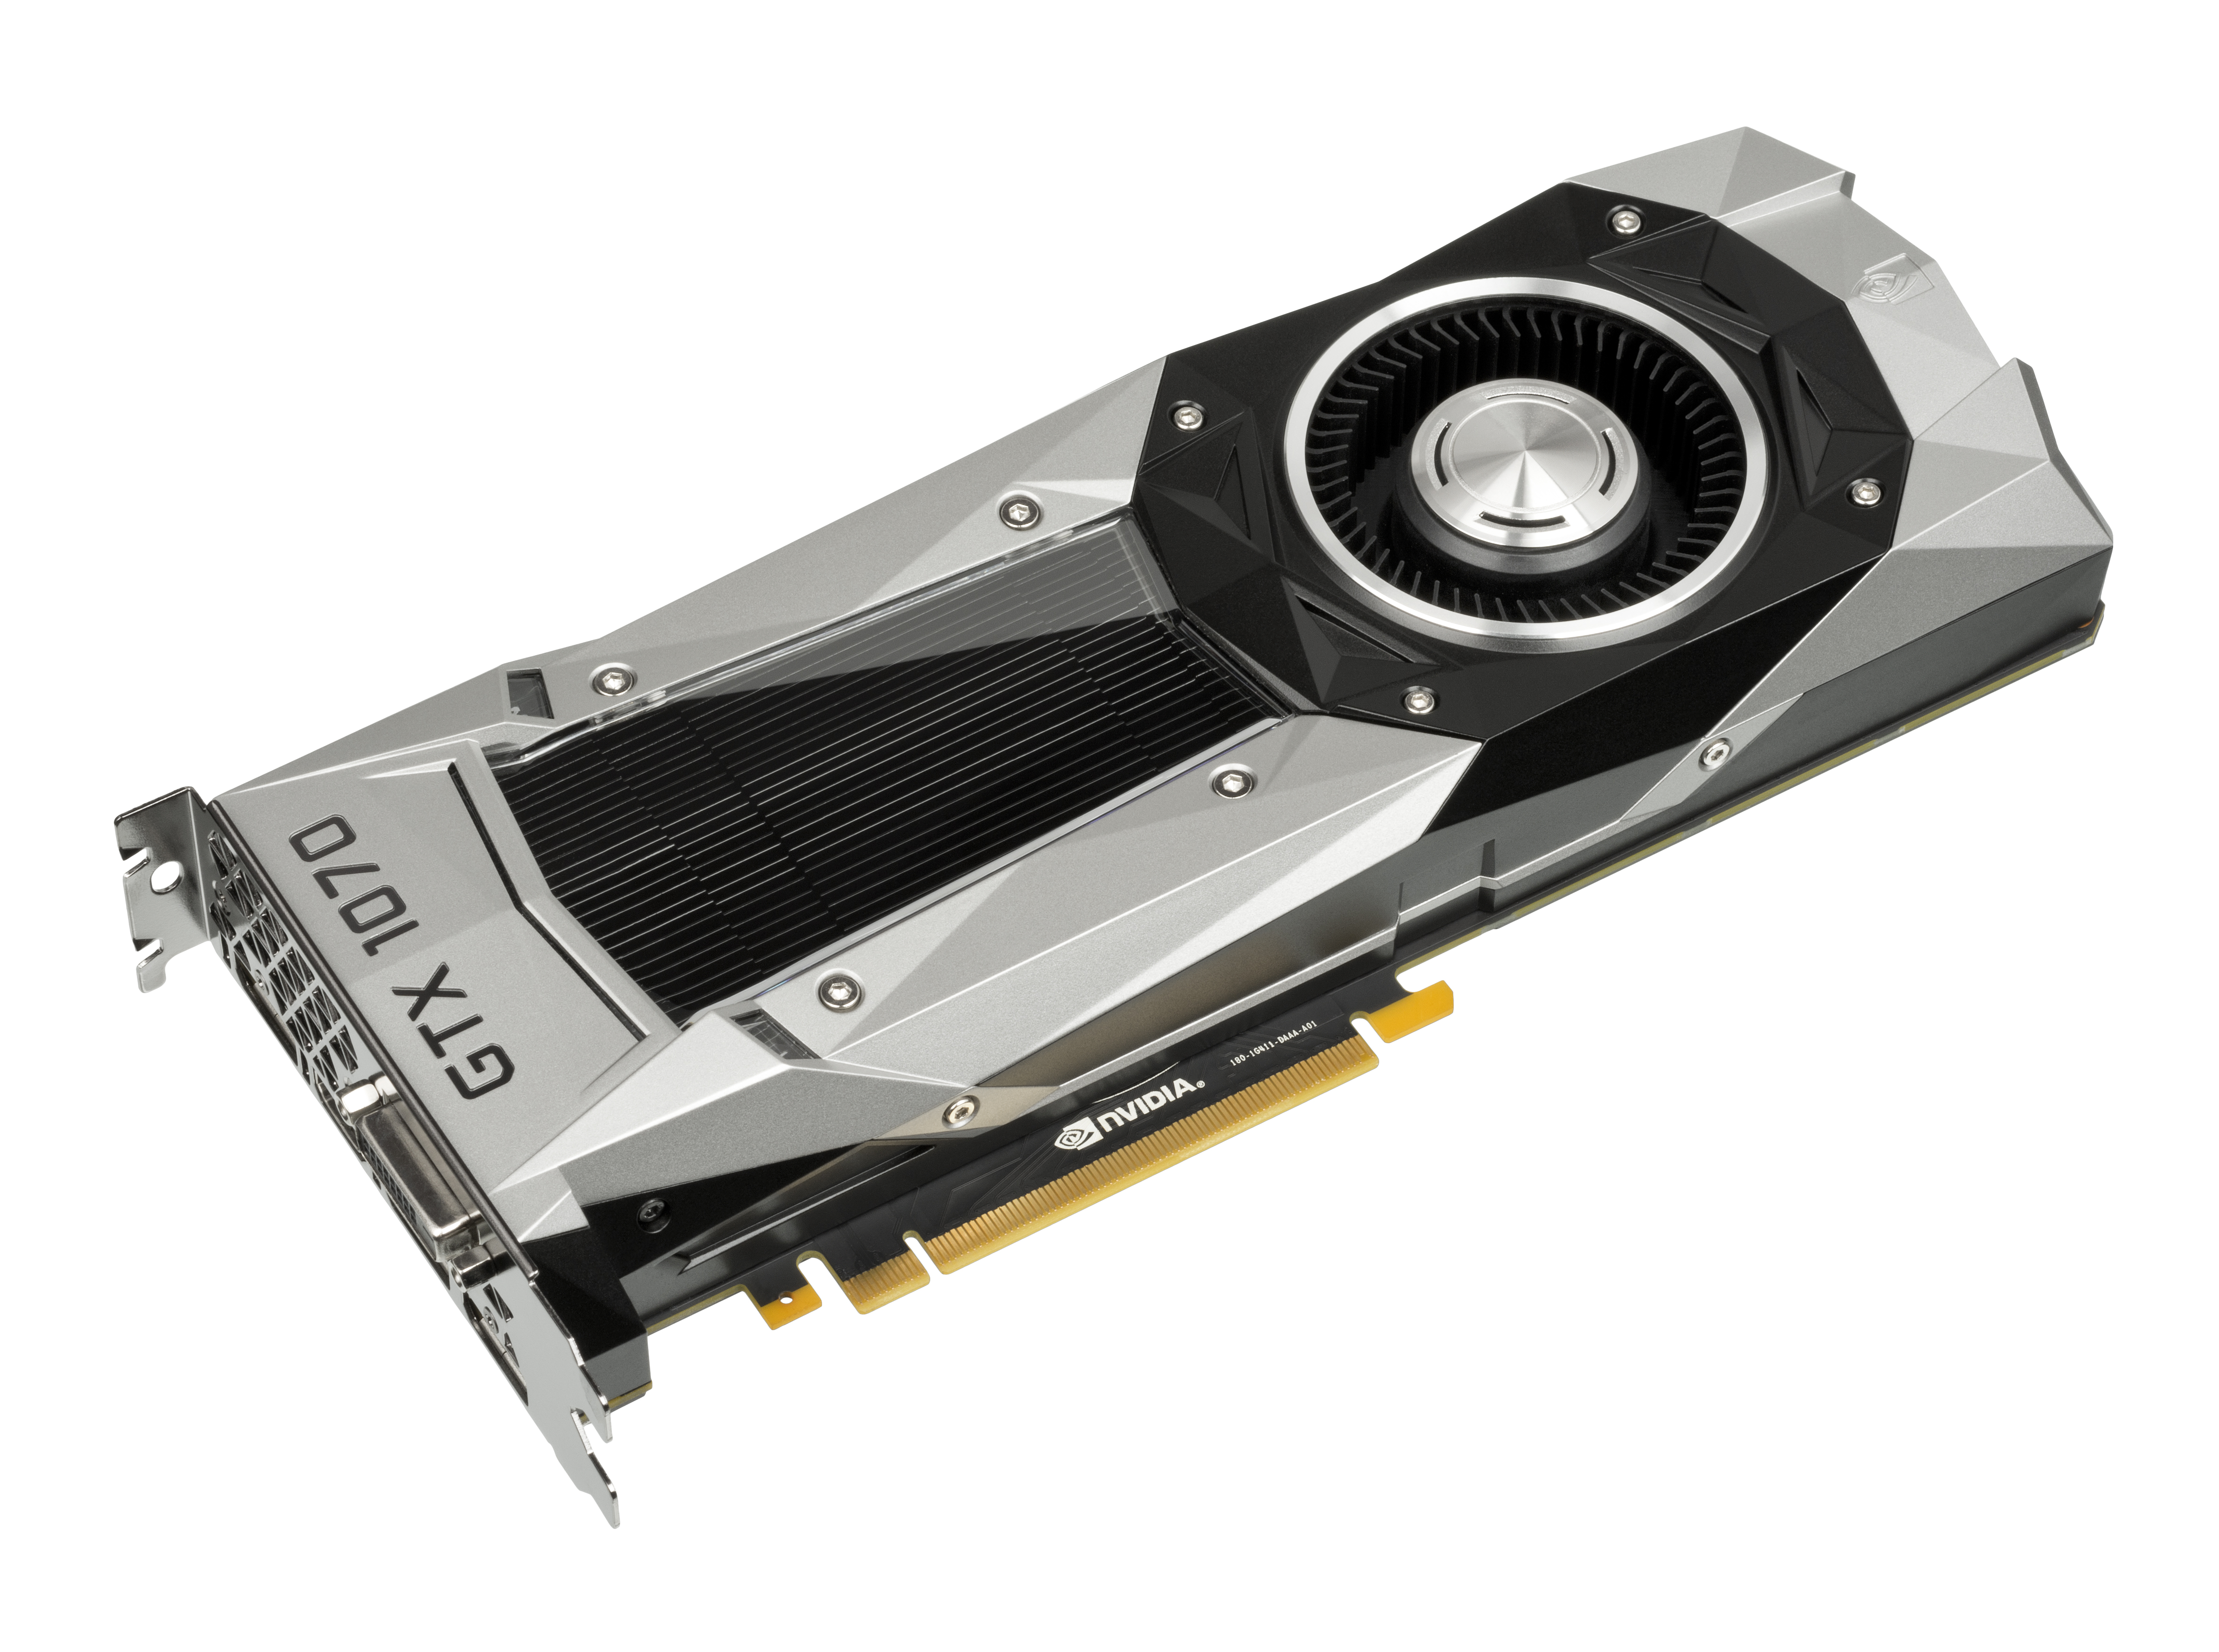
\includegraphics[width=.80\textwidth]{NVIDIA-GTX-1070-FoundersEdition-FL.jpg}
    \caption{Placa gráfica NVIDIA GTX 1070 para computadores de mesa "desktop", essa versão é a "Founders edition", possui cerca de 8 GBs de memória com uma banda de 256 GB/s , 1920 núcleos, frequência de funcionamento de 1506 MHz e consome 150W. (Fonte: Wikimedia Commons \protect\footnotemark)}
    \label{fig:gtx1070}
  \end{figure}

  \footnotetext{Disponível em \url{https://commons.wikimedia.org/wiki/File:NVIDIA-GTX-1070-FoundersEdition-FL.jpg} Domínio público}

  Placa de vídeo é uma peça que pode ou não estar presente em um computador, ela é responsável por fornecer o hardware especializado em renderização gráfica, projetado para prover um grande aumento de performance a um baixo custo se comparado a CPUs no que disrespeito a transformação de dados na memoria em imagens e vídeos, prontos para serem apresentados em telas e monitores. São constituídas principalmente de:
  \begin{itemize}
    \item Um chip de memória, cuja a principal função é armazenar texturas, ou qualquer outro dado que deverá ser várias vezes utilizado, consultado, no processo de renderização.
    \item Portas de acesso e conexão a monitores e telas, variam entre VGA (Video Graphics Array), DVI (Digital Visual Interface) e HDMI (High-Definition Muiltimidia Interface). São as saídas mais comuns às computações das placas.
    \item Um processador, uma GPGPU composta de alguns milhares de núcleos
    \item Uma ou várias ventoinhas, para dissipar o calor produzido pelo processador
  \end{itemize}

  A figura \ref{fig:gtx1070} é uma foto de uma placa gráfica da Nvidia, a NVIDIA GTX 1070, começou a ser comercializada em Junho de 2016 à um preço de 379 dólares e possuí 1920 núcleos de processamento à 1,506 GHz em sua GPU \citep{gtx1070:16}. Nessa mesma época também é comercializada o \textit{Intel® Core™ i7-6850K Processor} CPU da Intel, vendida na época a partir de 617 dólares, possui 6 núcleos à uma frequência de 3,6 GHz \citep{inteli7:16}. Um cálculo simples de tiques por segundo, ou seja, quantidade de ciclos que podem ser executados por segundo para cada processador demonstra que, enquanto a CPU da intel é capaz de realizar 21,6 bilhões de ciclos, no total, por segundo a GPGPU da nvidia é capaz de 2891,52 bilhões de ciclos, no total, por segundo, uma diferença de aproximadamente 133,8 vezes. A GPU que é 60,42\% do valor da CPU é mais de 100 vezes mais rápida.

  GPGPU é uma acrônimo para \textit{General Purpose Graphics Processing Unit} em tradução literal: Unidade de processamento Gráfico de Propósito Geral. É uma evolução, uma adaptação que as GPUs passaram, na qual sua cadeia de processamento gráfico foi flexibilizada tornado possível usá-la para propósitos mais gerais, indo muito além do escopo de produção de gráficos e imagens em três dimensões, porém suas origens e modo de operação advém da sua função original de processar uma cadeia de dados gráficos, e tal necessidade determinou qual seria o objetivo da arquitetura que tais processadores deveriam ter. Assim entender essa cadeia de processamento ou \textit{pipeline} dos dados das placas gráficas é importante para entender o por quê são como são \citep{massively:16}.

  O objetivo das GPUs é gerar imagens e vídeos que representam visões de uma cena virtual. A visão desta cena é descrita pela posição de uma câmera virtual e é definida pela geometria, orientação e propriedades materiais da superfície dos objetos na cena representados, bem como das propriedades das fontes de luz. APIs gráficas como OpenGL \citep{opengl}, DirectX \citep{directx} ou Vulkan\citep{vulkan} representam este processo como um pipeline que executa uma cadeia de operações sobre um conjunto de vértices enviados pela CPU, sendo que cada vértice possui propriedades determinadas, tais como cor, posição e vetor normal \citep{closer-look:08}.

  O vertex shader é uma parte integrante dessa cadeia e está no início do processamento.É um programa que executa um conjunto de operações sobre cada um dos vértices de entrada, projetando cada vértice, baseado em sua posição relativa à câmera virtual, em um anteparo 2D. Destes vértices, é montado um conjunto de triângulos, que representam os objetos no espaço 2D. Assim, quanto maior a quantidade de triângulos, melhor a qualidade com que o objeto será representado \citep{closer-look:08}. Visto que cada cena possui milhares de vértices e cada um deles pode ser tratado independentemente, os vértices podem ser processados de forma paralela e/ou distribuída \citep{gpu-comp:08}.

  O próximo passo é o processo de rasterização, consistindo em determinar quais espaços da tela são cobertos por cada triângulo. Esse processo resulta na geração de fragmentos para cada espaço de tela coberto. Um fragmento é o que virá a ser um pixel, que contém todas as informações necessárias para gerar uma imagem final como profundidade, posição no frame buffer, etc. A partir da localização da câmera virtual, os fragmentos que são ocultos por outros fragmentos são descartados, só é necessário mostras os objetos que podem ser vistos \citep{gpu-comp:08}.

  Por fim há o pixel shader que opera sobre a saída gerada pelo processo de rasterização. O pixel shader é um programa que consiste em um conjunto de operações que são executadas sobre cada fragmento, antes que estes sejam plotados na tela. Utilizando as informações de cor dos vértices e, possivelmente, buscando dados adicionais na memória global em forma de texturas (é nesse momento que a memória principal da placa é necessária), cada fragmento é processado para obter-se a cor final do pixel. Assim como na etapa de processamento de vértices, os fragmentos são independentes e podem ser processados em paralelo. Esta etapa é a que tipicamente demanda maior processamento dentro da estrutura do pipeline gráfico \citep{gpu-comp:08}.

  Uma vez que esses programas podem ser aplicados em milhares de vértices e pixels independentemente, as GPUs evoluíram para ser um conjunto de multiprocessadores massivamente paralelos. Além disso, dependendo do balanceamento da carga de trabalho das aplicações, apesar dos pixels serem dependentes dos vértices, ambos podem ser executados paralelamente. Esta característica resultou no aumento da programabilidade dos multiprocessadores da GPU \citep{massively:16}.

  Essa cadeia de processamento é o que destacou as GPUs das CPUs convencionais. No desenvolvimento de processadores dedicados a processar essa cadeia na forma mais eficiente possível as GPUs tomaram um caminho mais focado na paralelização, com mais núcleos, mais unidades logico-aritméticas em detrimento de mais ciclos por segundo, maiores frequências de trabalho, priorizando uma única memória grande e não muito rápida ao invés de varias camadas de memória cache muito rápida.

  Esta arquitetura muito focada, ganhou a atenção de outras computações não necessariamente ligadas a renderização de imagens. Tal demanda eclodiu na flexibilização das GPUs para GPGPUs.

\section{A História das GPU e GPGPU}
  As GPUs, a princípio, não foram criadas para cálculos numéricos ou simulações de partículas e sim para a renderização de imagens para jogos digitais, o alto custo na produção e aquisição de hardware mais potente, principalmente a memória, na década de 70 impulsionou a criação de processadores mais dedicados e com funções mais específicas para a renderização gráfica. Impulsionada pelo mercado de jogos de video game, e buscando evitar o alto valor de chips de memória, placas de sistemas de arcade apresentavam um conjunto de chips de vídeo para combinar os dados enquanto estes eram escaneados e direcionados ao monitor \citep{Hague:13}.

  Em 1977 o Atari 2600 usou um \textit{video shifter}, um tipo de circuíto integrado responsável por emitir o sinal de TV, chamado \textit{Television Interface Adaptor} ou TIA. Foi customizado para ser capaz de gerar as imagens finais para a tela, os efeitos sonoros e ler os comandos vindos dos joysticks, teve como direcionamento em seu design a economia de memória RAM, muito cara na época \citep{Hague:13} \citep{atari-field:83}.

  Em 1985 o Commodore Amiga apresentou um chip gráfico que vinha com um circuíto \textit{blitter}, para maior velocidade na manipulação de memória, transformação de bitmaps, desenho de linhas e funções de preenchimento de áreas. Também vinha com um coprocessador, capaz de executar instruções únicas e manipular os registradores em sincronia com o canhão de desenho dos tubos de raios catódicos das televisões \citep{amiga:17}.

  Na década de 90 a nintendo e a sony criaram seus consoles de vídeo game, o nintendo 64 e o playstation, ambos capazes de produzir gráficos em 3 dimensões a partir de polígonos. A distinção entre os dois principais processadores desses vídeo games eram claras, a nintendo já havia detalhado que seu sistema vinha com dois processadores: um de proposito mais geral o \textit{MIPS R4200} e o \textit{Reality Coprocessor} desenhado para cálculos em 3d de alta performance, pré-processamento de áudio e vídeo, mapeamento de textura e buferização de profundidade em tempo real \citep{manual64:98} \citep{N64Launch:96}.

  A nintendo não utilizou o termo CPU para descrever seu \textit{Reality Coprocessor}, foi a Nvidia em 1999 que popularizou o termo. Ele já existia desde década de 80, porém somente apos a campanha de marketing de sua placa de vídeo, a GeForce 256 com o logo: \textit{"the world's first GPU"} (A primeira GPU do mundo) que o termo ficou mais comum \citep{nvida256}.

  Em 2002 foi introduzido a placa de vídeo ATI Radeon 9700 (também conhecida como R300)\citep{AMD} nela tanto o pixel shader quanto o vertex shader poderiam implementar laços e longas contas aritméticas de ponto flutuante. A GPU foi se tornando tão flexível quanto as CPUs, porém em ordens de magnitude muito mais rápida em operações sobres listas, vetores.

  Em 2007 a Nvidia lançou a CUDA, uma extensão da linguagem de programação C que poderia ser compilada e executada na GPU, oficializando o início da programação heterogênea nas placas de vídeo. CUDA foi o primeiro modelo de programação para GPU amplamente adotada, logo no ano seguinte surgiu o OpenCL que se tornou amplamente suportado. OpenCL é um padrão aberto definido pelo \textit{Khronos Group} o qual permite o desenvolvimento de código tanto para a CPU quanto a GPU com ênfase na portabilidade \citep{opencl}. Programas nessa especificação podem rodar em dispositivos Intel, AMD, Nvidia e ARM.


  Já em 2014 a Nvida lança o GameWorks, um \textit{middleware} que facilita e aumenta a performance da renderização de partículas como fumaça e fogo, faz simulações de fluidos e cálculos de \textit{ray-tracing} ou rastreamento de raios \citep{gameworks}, enquanto a AMD lançou o TressFX, biblioteca que permite a criação de pelos e cabelos que aparência muito próxima a realidade \citep{tressfx}.

  \begin{figure}[!h]
    \centering
    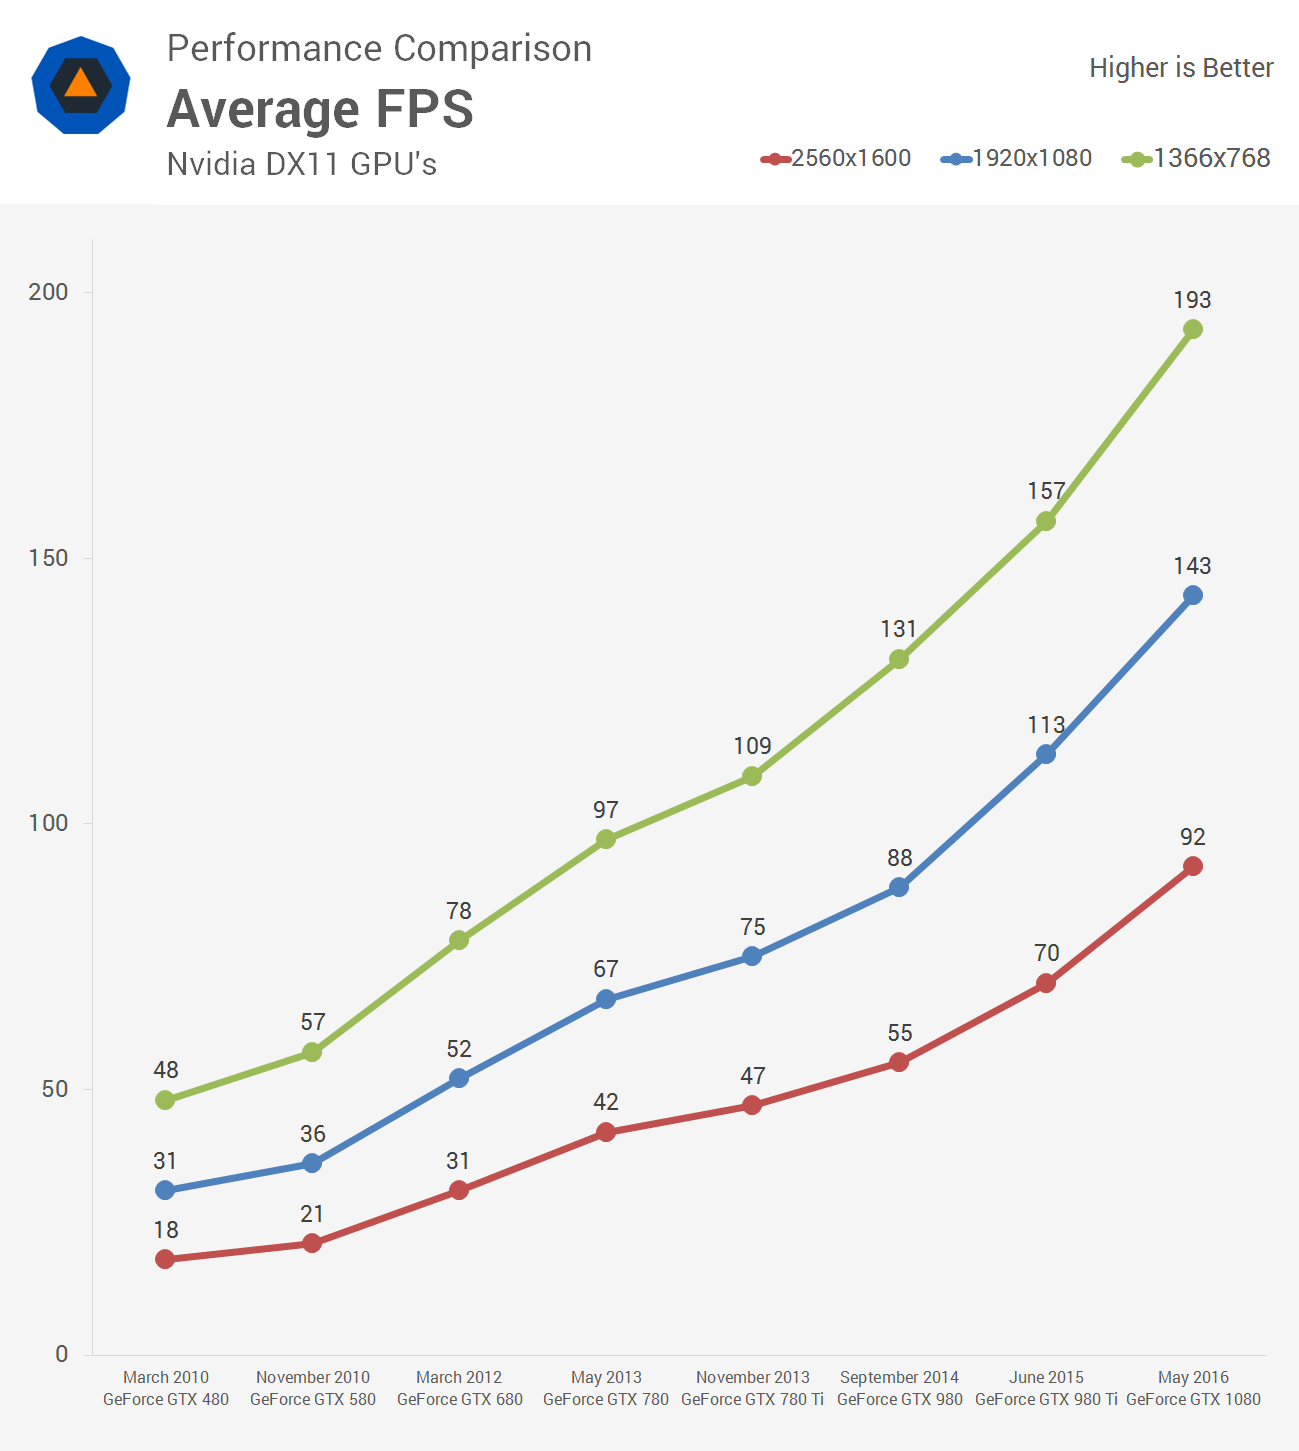
\includegraphics[width=.80\textwidth]{fpsXyear.png}
    \caption{média de fps (frames por segundo) em alguns jogo modernos para as principais placas de vídeo da Nvidia que foram lançadas de 2010 a 2016 . (Fonte: TECHSPOT \protect\footnotemark)}
    \label{fig:fpsXyear}
  \end{figure}

  \footnotetext{Disponível em \url{https://www.techspot.com/article/1191-nvidia-geforce-six-generations-tested/page6.html} visitada em 31/01/2018}

  O gráfico \ref{fig:fpsXyear} demonstra a performance de algumas das principais placas de vídeo da Nvidia em um período de 6 anos, de 2010 a 2016. O gráfico demonstra a tendencia ainda muito forte de crescimento cada vez mais veloz da performance das GPUs ao longo do tempo, como a demanda para processamento e performance gráfica é virtualmente infinita e além disso a cada nova versão a diferença da atual para a anterior é cada vez maior, não há previsão para o esfriamento na produção e desenvolvimento de GPUs mais e mais poderosas.

\section{CPU vs GPU}

  Ambos os processadores tem a tarefa primordial de executar instruções manipulando a memória e performando cálculos aritméticos, porém suas necessidades particulares e os casos de uso que se encontraram redefiniram sua arquitetura, agora mesmo tendo a mesma origem suas peças de hardware são profundamente distintas, cada uma com suas vantagens e desvantagens sobre a outra.

  Já em 2009, o poder computacional para operações em ponto flutuante de uma GPU era cerca de dez vezes maior ao de uma CPU, ver seção ~\ref{sec:video_boards}. Já a sua taxa de transferência era cerca de três vezes superior \citep{massively:16}. Uma CPU é otimizada para desempenho de código sequencial, geralmente utilizam-se de uma lógica de controle mais sofisticada, fazendo com que a CPU seja projetada com mecanismos como previsão de desvios e execução fora de ordem (Out-of-order execution (PDF). cs.washington.edu. 2006. Retrieved 17 January 2014. "don't wait for previous instructions to execute if this instruction does not depend on them"). Desta forma, permite-se que um único fluxo de instruções seja executado em paralelo enquanto a aparência de uma execução sequencial é mantida. Além disso, a CPU também é otimizada de forma a reduzir a latência de acesso aos dados e às instruções na memória principal. De fato, grande parte dos recursos da CPU são utilizadas para o gerenciamento de vários níveis de memória cache, que possuem o objetivo de minimizar o tempo necessário para que os dados requisitados sejam de fato utilizados pelo processador. Uma vez que a CPU tem como alvo programas de propósito geral, poucos de seus recursos são utilizados para processamento de operações de ponto flutuante \citep{massively:16}.

  Já a GPU foi concebida para ser a solução de problemas no qual processamento dos dados pode ser realizado massivamente em paralelo, ou seja, o mesmo programa é executado simultaneamente em muitos conjuntos de dados com alta intensidade aritmética (NVIDIA, 2010a). Por causa disto, as GPUs dedicam a maior parte de seus recursos ao processamento aritmético ao invés de cache de dados ou controle de fluxo \citep{massively:16}.

  Na Figura~\ref{fig:cpuvsgpu}, é exposta de maneira simplificada com que os transistores do hardware são distribuídos nos chips da CPU e GPU. Na imagem da esquerda há a representação de uma CPU, nela grande parte da área do chip é dedicada à memória cache e a lógica de controle. já na GPU, a imagem do lado direito, a maior parte dos recursos do chip é destinada ao processamento em paralelo de operações em ponto-flutuante. Assim, sua capacidade de processamento de dados é potencializada consideravelmente \citep{NTesla:16}.

  Na GPU, grande parte dos dados é utilizada uma única vez, sendo que estes dados precisam ser transferidos da memória principal da GPU para o uso de seus multiprocessadores. Desta forma, o sistema de memória da GPU é projetado para maximizar a taxa de transferência de dados (throughput), ou seja, a GPU é projetada de forma a aumentar a largura de banda, ao invés de minimizar a latência para o acesso aos dados. Esta grande largura de banda é obtida através do uso de amplos barramentos e memórias dynamic random access memory (DRAM) do tipo graphics double data rate (GDDR) \citep{closer-look:08}. É importante destacar que nem todas as aplicações terão um desempenho melhor na GPU em relação à CPU. As GPUs são projetadas como engines de processamento numérico, e não executam bem os programas sequenciais que as CPUs normalmente executam. Assim, deve-se utilizar a placa GPU como um coprocessador para auxiliar a CPU na execução dos programas, de forma que sejam atribuídas as partes sequenciais à CPU e as partes com processamento paralelo aritmético à GPU \citep{massively:16}.

  \begin{figure}[!h]
    \centering
    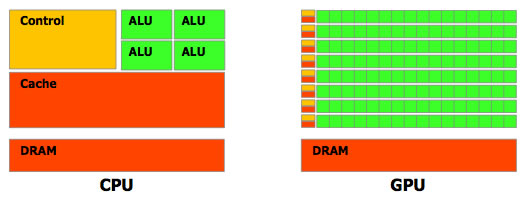
\includegraphics[width=.80\textwidth]{comparacao_GPU_CPU.png}
    \caption{Imagem comparando de forma simplifica a arquitetura dos processadores. Do lado esquerdo a arquitetura de uma Unidade de Processamento Central, muito espaço para o cache e a unidade de controle. Do lado direto uma unidade de processamento Gráfica, como uma grande região segmentada dedicada a computação aritmética e lógica. (Fonte: Wikimedia Commons \protect\footnotemark)}
    \label{fig:cpuvsgpu}
  \end{figure}

  \footnotetext{Disponível em \url{https://commons.wikimedia.org/wiki/File:Cpu-gpu.svg} Creative Commons Attribution 3.0 Unported}

\section{Bibliotecas: OpenCL e CUDA}

  Nos primórdios da computação genérica em GPUs duas formas principais surgiram para lidar com essa programação, a linguagem CUDA e a OpenCL.

  Open Computing Language (OpenCL) é um arcabouço, um \textit{framework}, aberto para programação genérica para vários processadores, não só GPGPUS como também CPUs e outros dispositivos focados em processamento. O OpenCL da suporte para sistemas embarcados, sistemas pessoais, corporativos e até de Computação de Alta Performance. Isso é alcançado graças a criação uma interface de baixo nível, ou seja, o mais próximo do hardware possível, mantendo um auto desempenho, com uma abstração portátil. O OpencL também é uma API para controle de aplicações paralelas em sistemas com processadores heterogêneos. O OpenCL consegue, numa mesma aplicação, reconhecer vários processadores e dispositivos diferentes dentro de um mesmo computador, ou cluster de computadores, e executar códigos distintos entre eles, coordenando os dispositivos. Desta forma, igual ao CUDA, a parte do código que é executada sempre na CPU, de forma sequencial é chamada de código \textit{Host}. A parte que roda o \textit{kernel}, o código que geralmente roda na GPGPU, preparado para rodar massivamente em paralelo é chamado de \textit{device} . É importante lembrar que dado essa generalização do OpenCL, é possível que a CPU onde o código do host esteja executando seja também usada para rodar um kernel, e essa CPU passa a executar código device ao mesmo tempo em que roda código host. Tanto o fato do OpenCL ser aberto quanto o fato dele não se restringir a um hardware especifico fazem dele a linguagem mais usada para GPGPU fora de GPUs NVIDIA \citep{EDOpencl:11}.

  Compute Unied Device Architecture (CUDA) pode ser descrita como uma linguagem de programação para GPGPUs criada pela NVIDIA em 2007 para seus processadores G80, fornecidos nas placas GeForce 8800 Ultra, GeForce 8800 GTX, GeForce 8800 GTS(G80). Ele adiciona suas diretrizes para as linguagens C, C++, FORTRAN e Java, permitindo que elas usem a GPGPU. Esse trabalho usa o CUDA junto com a linguagem C.

  A versão 1.0 do CUDA foi disponibilizada em Fevereiro de 2007. Atualmente só existe um compilador para CUDA, o nvcc, e ele só da suporte para GPUs NVIDIA. Para uma função executar na GPGPU esta precisa ser invocada de um programa da CPU. Chamamos esse programa de Host e a GPGPU onde o kernel executará de Device. O CUDA implementa um conjunto virtual de instruções e memória, tornando os programas retroativos. O compilador primeiro compila o código em C para um intermediário, chamado de PTX, que depois será convertido em linguagem de máquina. Na conversão do PTX para linguagem de máquina o compilador verifica quais instruções o device suporta e converte o código para usar as instruções corretas. Para obter o maior desempenho possível, é importante saber para qual versão o código final será compilado, pois na passagem do código de uma versão maior para uma menor não existe a garantia que o código seguira as mesmas instruções, o compilador pode mudar um conjunto de instruções para outro menos eficiente, ou em alguns casos, algumas instruções não existem em versões mais antigas.

  Uma grande diferença entre essas duas linguagens é a quantidade e qualidade da documentação e recursos para o seu aprendizado. As duas apresentam basicamente a mesma estrutura e modelo de desenvolvimento, tornando razoavelmente simples para uma programadora ou um programador migrar de uma linguagem para a outra, porém a grande diferença nos recursos de aprendizado e documentação entre as duas, torna consideravelmente mais fácil e rápido aprender e desenvolver primeiramente com a linguagem CUDA.

  Este é o principal motivador para que se tenha escolhido a linguagem CUDA para aumentar a performance do grmonty. O nosso grupo de estudos que é focado em aprimorar o grmonty tem a necessidade de ter um conjunto de pessoas com certo domínio sobre a linguagem que será usada no desenvolvimento, e graças a facilidade e agilidade do aprendizado da linguagem CUDA esta foi a escolhida que ser primeiramente empregada no aprimoramento de performance do grmonty.

\section{Aplicações e usos avançados}

  No ano de 2017 não esta se observando uma retração no desenvolvimento das GPUs e sim uma expansão. Seja provocada pelo já conhecido mercado de jogos digitais, seja por novas fronteiras como mineração de cripto-moedas ou novas técnicas de aprendizado de máquina como \textit{deep learnig}. Abaixo são citadas algumas das aplicações e modelos de problemas que expandem o escopo e avançam o potencial que as GPUs podem alcançar.

  O aprendizado profundo, \textit{Deep Learning} é uma área de grande crescimento em inteligência artificial, ajudando os desenvolvedores a terem um controle mais fino e compreender melhor dados, como imagens, som e texto. Usando redes neurais, esses sistemas têm a capacidade de ver, aprender e reagir a situações complexas tão bem quanto ou melhor que os humanos treinados em tais ações. Isso está levando a uma forma totalmente diferente de pensar sobre coleta dados, tecnologias, produtos e serviços que podem ser oferecidos.

  As soluções de aprendizado profundo contam quase exclusivamente com a computação acelerada pelas GPGPUs para treinar e acelerar aplicações, como identificação de imagens, caligrafia e vozes. As placas gráficas se destacam em pipelines paralelos e aceleram as redes neurais em até 10 a 20 vezes, reduzindo cada uma das muitas iterações de treinamento de dados de semanas para dias. As placas de vídeo têm acelerado o treinamento de redes neurais profundas em 50 vezes em apenas três anos — mais rápido do que a lei de Moore — com outras 10 vezes previstas para os próximos anos. A inovação nessa área está acontecendo a um ritmo acelerado, abrindo oportunidades em aplicações como robótica, medicina e carros auto-dirigíveis.


  A realidade virtual (VR) é uma forma mais profunda de simular cenários mais realistas. Normalmente usando-se de capacetes ou óculos específicos, as vezes em combinação com objetos físicos reais no ambiente, imagens são geradas para cada um dos olhos e são atualizadas conforme o usuário move sua cabeça, proporcionando a sensação de estar corporalmente presente na cena gerada por computador. A pessoa portando esse equipamento pode "olhar ao redor" e interagir com itens e propriedades do mundo virtual.

  O processamento necessário para gerar estas cenas de realidade virtual é atualmente muito alto, normalmente sendo exclusivos de dispositivos de primeira linha, uma vez que para que ocorra uma experiencia razoavelmente imersiva se faz necessário haver um atraso desprezível na captação e apresentação das imagens, de acordo com o movimento do usuário, e as imagens devem ser atualizadas a uma frequência altíssima para que não ocorra enjoes da parte de quem usa tais aparelhos.

  O processo de mineração de criptomoedas pode ser extremamente lucrativo se for feito de maneira muito rápida, uma vez que quanto mais blocos da \textit{blockchain} você processar maior a sua chance de ganhar uma moeda no processo. Com o crescimento do interesse em bitcoins minerados - pessoas que buscam processar a blockchain, realizando transações das moedas - concluíram que as GPUs das placas gráficas usadas primordialmente para jogos poderiam ser usadas para resolver de forma muito mais rápidas os hash necessários para processar a blockchain.


  A busca e o empenho dos mineradores em performar da melhor forma possível, empurrou o desenvolvimento das GPGPUs à criação de novas arquiteturas de placas gráficas e até a novos tipos de GPUs, quase ou nada focadas em gráficos. Esses novos dispositivos focados em mineração de criptomoedas se tornaram um novo foco de desenvolvimento e inovação na área de processadores massivamente paralelos de computação genérica, ou mais especificamente na resolução de hashes ou fatoração de números primos.
